\chapter{Method}

This chapter describes \ldots compares \ldots


\section{Software development methodology}

Some features of of agile software development processes, such as pair programming in Extreme Programming \cite{xpparr} and meetings in Scrum [], are only relevant to the developing software in teams, and are therefore not relevant to this solo effort. \ldots

However, other principles are applicable, such as valuing ``Working software over comprehensive documentation'' [[agile manifesto]]. Artoo is 

Gerald Jay Sussman gave a talk entitled ``Why programming is a good medium for expressing poorly understood and sloppily formulated ideas'' \ldots


Another consideration is the role of the product owner, typically a customer or boss \ldots 





\section{The structure of Artoo}

Artoo consists of some separate parts:

\begin{description}

\item[{\tt SVGGraph}] A representation of a domain graph -- not necessarily a GSN argument.
This consists of SVG shapes, most of which are graph nodes containing textual labels in the form of SVG {\tt ForeignObject}s; and SVG paths representing the graph's directed edges.
The shapes can be moved around the canvas by clicking and dragging, and the edges appear as automatically drawn quadratic B\'{e}zier curves. 

Although this abstraction is described as ''general SVG graph tool code'', the scope of the features included in it appears to anticipate GSN-specific use. Clear examples of this are the ability to attach diamonds to shapes (which can representing undeveloped parts of the argument), the notion of connections being either horizontal (anticipating the GSN's InContextOf relationship) or vertical, and the particular SVG shapes on offer (rectangle, rounded rectangle, rhomboid, ellipse, etc. -- all happen to correspond with types of GSN element).

\item[{\tt GSNGraph}] A wrapper around {\tt SVGGraph}, containing additional methods and data structures [to cloak it with GSN-specific terminology]: for example, {\tt markNodeUndeveloped(id)} makes use of {\tt SVGGraph}'s {\tt addDiamondToShape(id)} method, but also updates the `undeveloped' property of the {\tt GSNGraph}'s own representation of the node.

\end{description}
  
Alongside this is other functionality, such as the ability to export PNG images of arguments, and the user interface with menus and dialog boxes to facilitate creating GSN arguments and generally using the tool. Further description of all the files ica


\section{Requirements and scope}

Informed by the findings of research discussed in chapter~\_, and the context of the existing Artoo software, some requirements can be specified.

The presence of layers of abstraction -- GSN graphs layered upon more general graphs -- might be feasibly followed through in implementation of automatic layout: first implementing a more general layout algorithm, and then  extending it to address the specific requirements of the GSN domain. However, what the practical difference would be is moot. The most prominent extra requirement of GSN argument layout is the placement of contextual elements horizontally beside their parents, but this notion of connections being either horizontal or vertical is already built into the general {\tt SVGGraph} model. The direction of relationships is also part of {\tt SVGGraph} -- supporting undirected graphs would entail an additional property to indicate that an edge's direction should be ignored. In fact, this suggests that {\tt SVGGraph} should but the more ``general'' graph layout feature will happen to 

One insight from [[Purchase]] was that authors do not distinguish between the activities of layout and [editing/creating], and the conclusion that tools should [combine them]. 


Artoo also allows the drawing of invalid GSN arguments ...
if the graph layout [thing] is to be executed every time the graph is edited, \todo{see one of the recommendations from \cite{5674033}} then it must accept these .
If the algorithm [is exposed to the user by a] button, then there is the possibility of checking a structure's validity; however, partr



\subsection{Good layout}


\subsection{Speed}


\citeauthor{Miller:1968:RTM:1476589.1476628}'s  user perceives an interactive system to be working if it responds \ldots and broken if it takes \_ or longer.



\subsection{Technical}

Already, Artoo only works a limited set of web browsers: recent versions of \ldots
The features added in this project will not interact with the browser in any new way -- only needing to change the position of nodes, using methods already in the code -- it is very unlikely that there will be any problems \ldots



\section{Experimental methodology}


\subsection{Test data}

\begin{itemize}
    \item Four graphs from \citet{aldenthesis}
\end{itemize}

Up to a point, GSN arguments are quite homogeneous. 


\section{Springy}

Springy.js is an existing JavaScript implementation of a force directed graph drawing algorithm.
It lays out graphs by representing nodes as point charges and edges as springs. Springy.js simulates the electrostatic forces of interaction between these point charges, and the extension of the springs caused by these forces, according to Coulomb's and Hooke's laws.



\begin{description}

\item[Hooke's law] Hooke's law describes the relationship between the force exerted on a spring,
    and the distance by which it extends as a result of that force being exerted.
    It states that the distance is proportional to the force:

    $$
    F = -kX
    $$

    (where $F$ is the force exerted on the spring,
    $X$ is the distance by which it extends,
    and $k$ is a constant representing the spring's stiffness)

\item[Coulomb's law] Coulomb's law describes the electrostatic force of interaction between two point charges.

    ``is directly proportional to the scalar multiplication of the magnitudes of charges and inversely proportional to the square of the distance between them.''

    ``The force is along the straight line joining them.
    If the two charges have the same sign,
    the electrostatic force between them is repulsive;
    if they have different sign,
    the force between them is attractive.'' \todo{reference}

    In scalar form:

    $$
    |\mathbf F|=k_e{|q_1q_2|\over r^2}\qquad
    $$

    (where $F$ F is the $q_1$ and $q_2$ are the two charges, $r$ is the distance between them, and $k_e$ is Coulomb's constant 

    In vector form:

    $$
    \qquad\mathbf F_1=k_e\frac{q_1q_2}{{|\mathbf r_{21}|}^2} \mathbf{\hat{r}}_{21},\qquad
    $$

    Coulomb's law closely resembles Newton's law of universal gravitation, which describes the gravitational force between two masses.
    But gravitational force is always attractive (if it is assumed that nothing can have negative mass),
    whereas the electrostatic force described by Coulomb's law can be repulsive (if both particles' charges have the same sign)

\item[Newton's laws of motion] Finally

\end{description}

The work of [[Eades and others]] suggests that

\subsection{Implementing }

Springy, as distributed online\footref{fn:springy}, consists of a layout algorithm implemented in JavaScript (springy.js) along with a sample rendereer for displaying a graph layout 

[[screenshot]]



\section{Arbor}

Simple though the brute-force force directed algorithm implemented in Springy is to understand, it also inefficient.

The Barnes-Hut algorithm is $O$



\section{Layered}

A key part of the layered layout approach is notion that directed graphs flow in a single direction (typically from top to bottom or from left to right). This is highly applicable to GSN arguments, particularly as specified by the GSN community standard document's guidelines \cite{gsnstandard}. The layout's 





Figure~\ref{fig:dagre1} shows

\begin{figure}
  \centering
  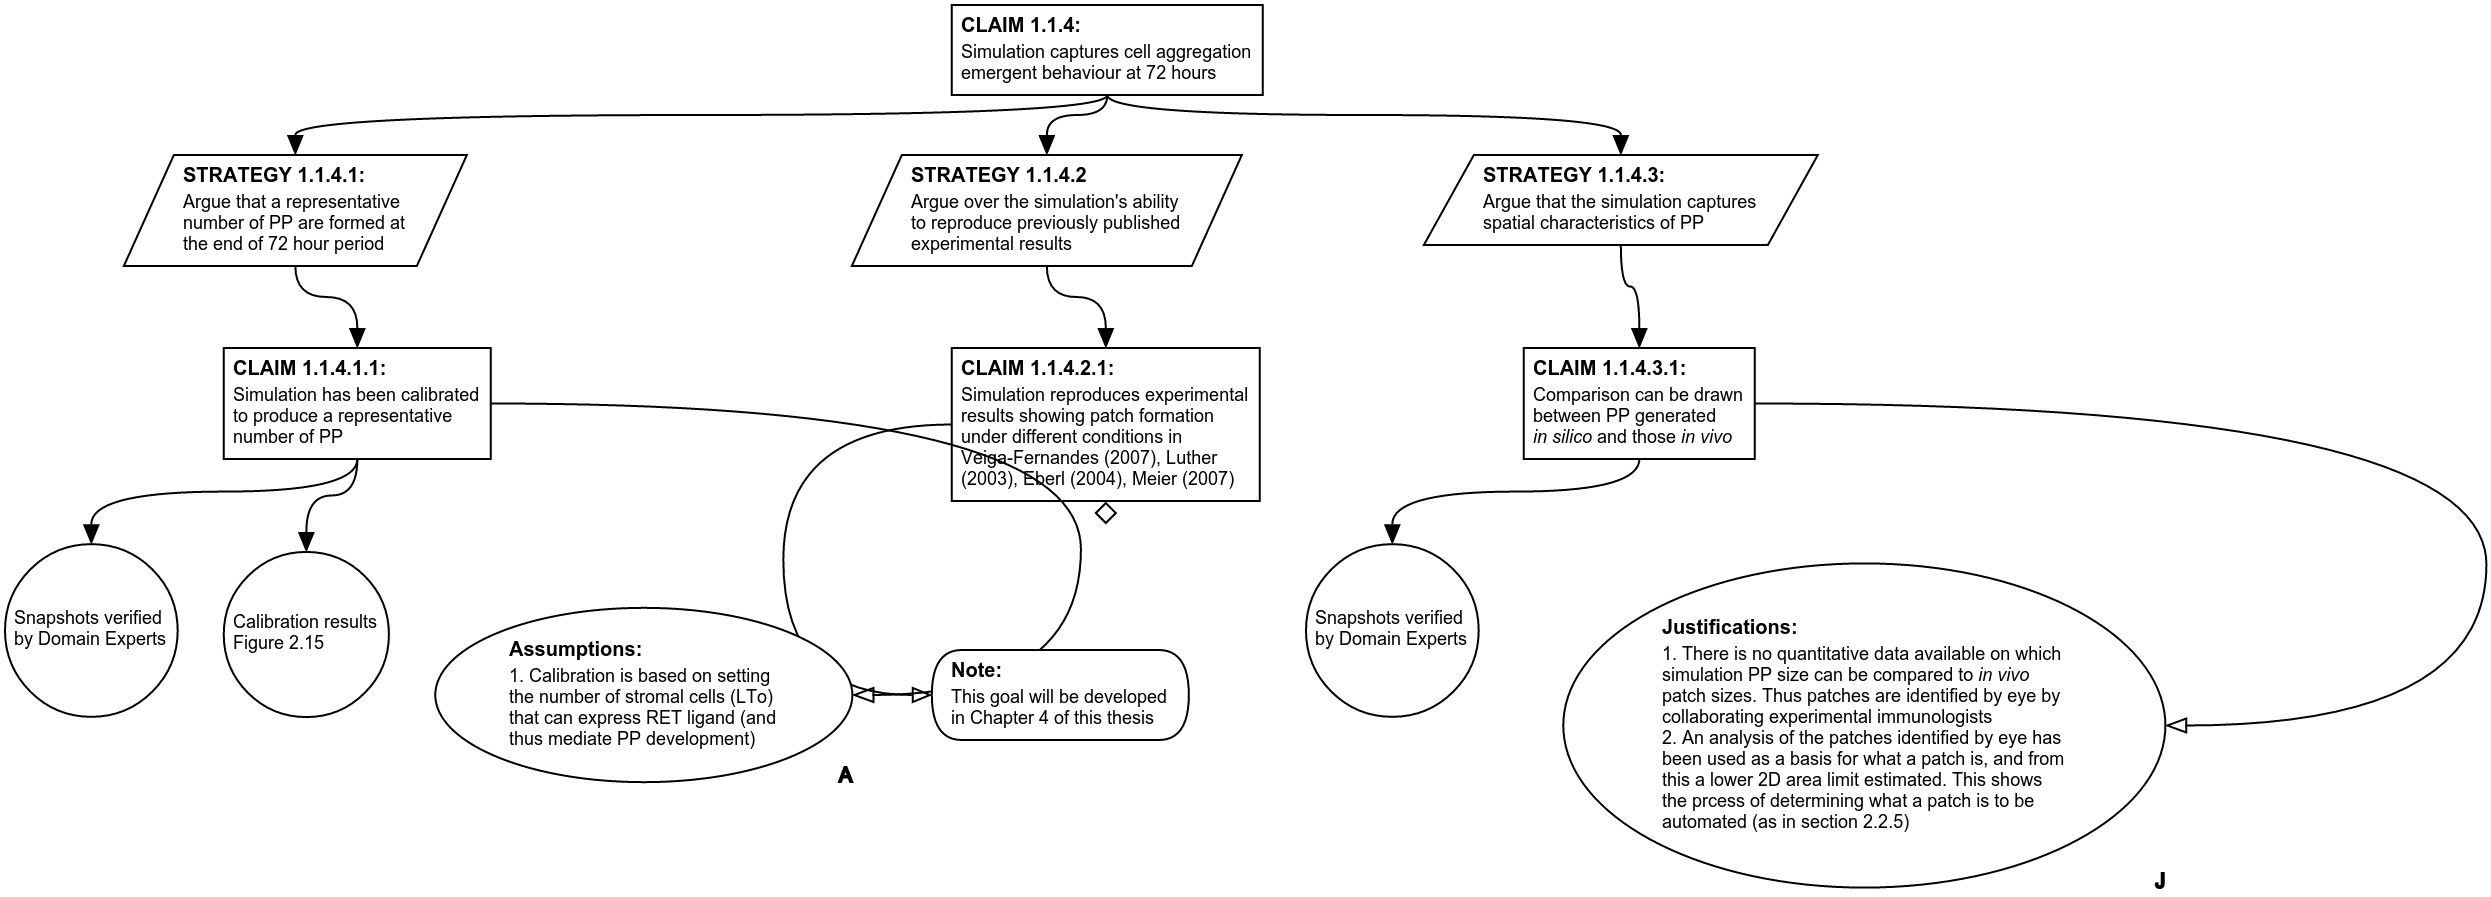
\includegraphics[width=\textwidth]{graphics/results/dagre.png}
  \caption{A na\"ive use of Dagre to render a graph from \cite{aldenthesis}}
  \label{fig:dagre1}
\end{figure}



\begin{figure}
  \centering
  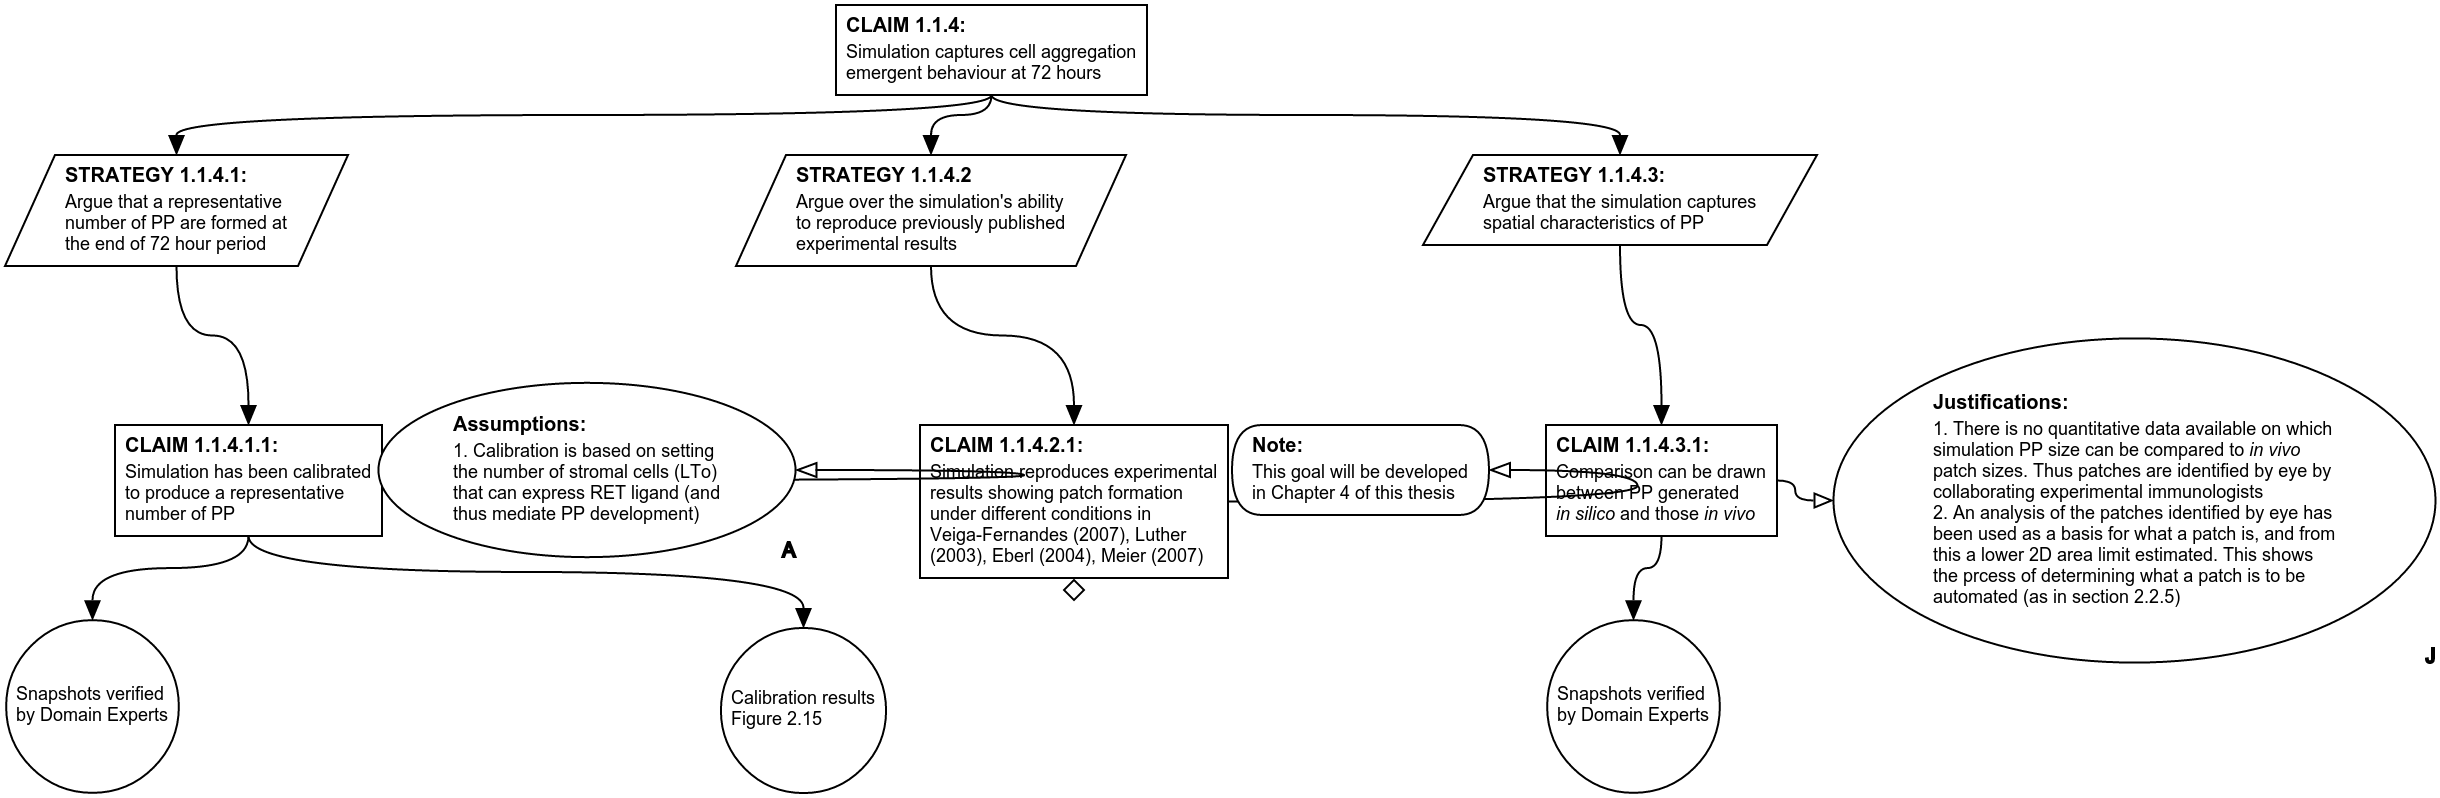
\includegraphics[width=\textwidth]{graphics/results/dagre-enhanced.png}
  \caption{A less na\"ive use of Dagre compared to figure~\ref{fig:dagre1}, with context, assumption and justification elements placed to the sides through the use of unrendered dummy elements}
  \label{fig:dagre2}
\end{figure}



\begin{landscape}

\section{Testing}



\subsection{Results}

\subsubsection{Dagre}

\begin{tabular}{ | c | c | c | c | }
    \hline
    Graph & Area & Running time & Edge crossings \\
    \hline
    1     & & & \\
    \hline
    2     & & & \\
    \hline
    3     & & & \\
    \hline
    4     & & & \\
    \hline
\end{tabular}



\end{landscape}


\subsection{Requirements validation}


